\chapter{Introduction}
\graphicspath{{./Introduction/img/}}
\section{Robot Operating System (ROS)}
  
\begin{figure}[h]
	\centering
	
\includegraphics[scale=2]{ROS_LOGO.pdf}
	\caption{ROS Logo}
\end{figure} 

The Robot Operating System or short ROS is a meta operating system from WillowGarage which is designed for usage with distributed 
robot systems. It's called a meta operating system because it needs another operating system to run. It's mainly developed for Ubuntu 
(a Linux distribution) but it also supports other Operating Systems like Windows and Mac OS, but the support for them can still be considered 
as experimental. 

It also works together with a Google Android device by runnning a special software which makes the device available
as hardware extension, enabling processes on different machines to access cameras, accelerometers and the display.
The basic underlying principle of ROS is the Publisher Subscriber Pattern further called PSP is a pattern which 
implements the realworld behaviour of publishers and subscribers (e.g. newspaper) in software. 
The publishing house advertises and publishes its newspaper or magazine while the subscribers look at the advertisements
and subscribe to the newspaper like seen in figure \vref{figure:psp_real}.

\begin{figure}[h]
	\centering
	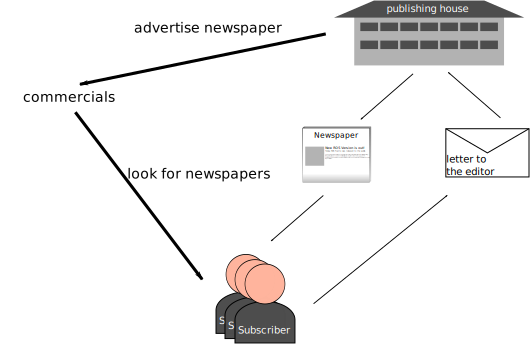
\includegraphics[scale=0.7]{PS_Newspaper.pdf}
	\caption{Publisher Subscriber Priciple in Reality}
	\label{figure:psp_real}
\end{figure} 

In the PSP the newspapers are now called topics. A PSP system is a subset of different applications, those applications are called nodes.  
Each node can publish or subscribe multiple topics at the same time. So it is possible to create a network of different nodes which
do processing or act as user interface. The advertisements of the real world are replaced by a so called master. 
The master knows everything about the communication channels, all nodes, the computer they run on and 
which topics they subscribe and publish. When a new node starts up, it checks for other nodes publishing or subscribing the relevant topics
and connects with them. An example of this is shown in figure \vref{figure:psp_ROS}.
In the picture there are different nodes for the robots running gear, its laserscanner, the motion planing system and the graphical user interface.
connected together by topics.

\begin{figure}[h]
	\centering
	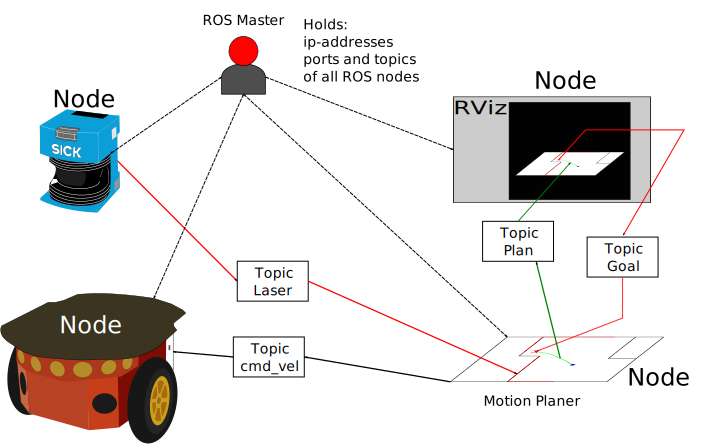
\includegraphics[scale=0.6]{PS_ROS.pdf}
	\caption{Publisher Subscriber Pattern in ROS}
	\label{figure:psp_ROS}
\end{figure} 


 
\clearpage


\section{Kinect}

\begin{figure}[h]
	\centering
	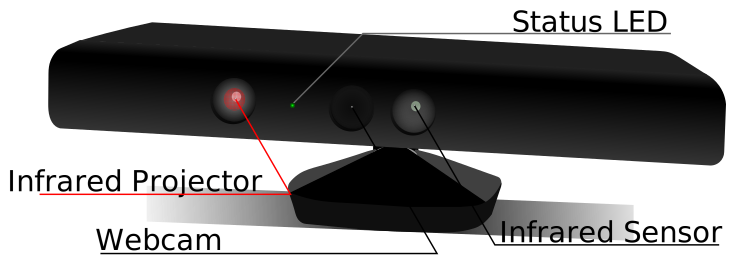
\includegraphics[scale=0.7]{Kinect.pdf}
	\caption{Microsoft Kinect Camera Overview}
	\label{figure:kinect_ir}
\end{figure}

The Kinect is a combination of a standard color camera and a depth sensor produced by Microsoft. The depth sensor is made by Primesense and 
it's working principle is currently a secret of the manufacturer. The known facts are, that the Kinect uses an ir-projector to draw a 
grid of very small points onto each surface (see figure \vref{figure:kinect_ir})on its front and a ir-camera to process the result somehow.  
There are different approaches on how it might work, the most resonable is that it uses 
specific groups of points and their position on the resulting camera image to calculate how far 
away they are like a laser scanner (in figure \vref{figure:ls_WP}) but in three dimensons (see figure \vref{figure:kinect_WP}) 
than in two dimensions. 

\begin{figure}[h]
	\centering
	\includegraphics[scale=1]{ir_kinect.png}
	\caption{Kinect IR Sensor Image}
	\label{figure:kinect_ir}
\end{figure}

\begin{figure}[h]
	\centering
	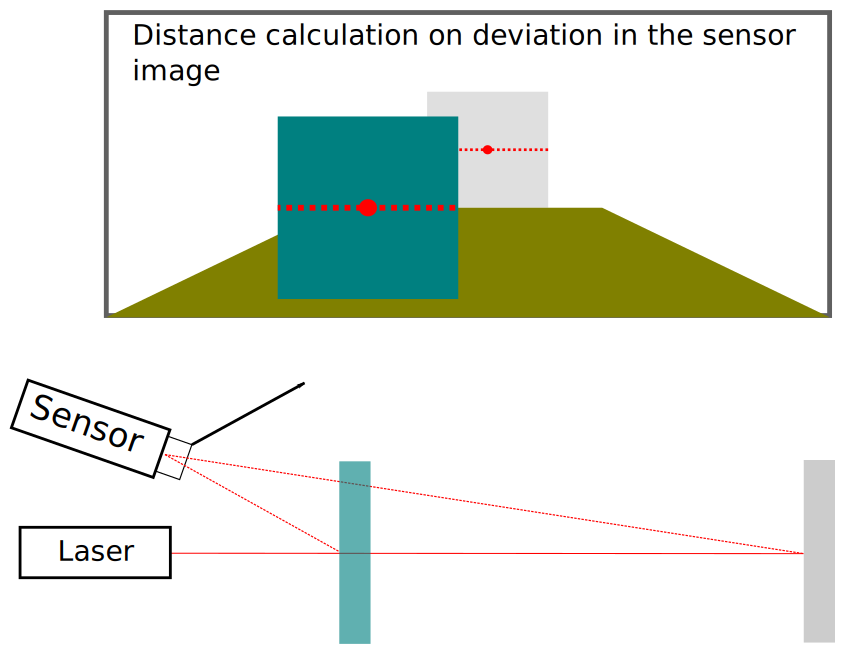
\includegraphics[scale=0.5]{laserScannerPrinciple.pdf}
	\caption{Laser Scanner Working Principle}
	\label{figure:ls_WP}
\end{figure}


\begin{figure}[h]
	\centering
	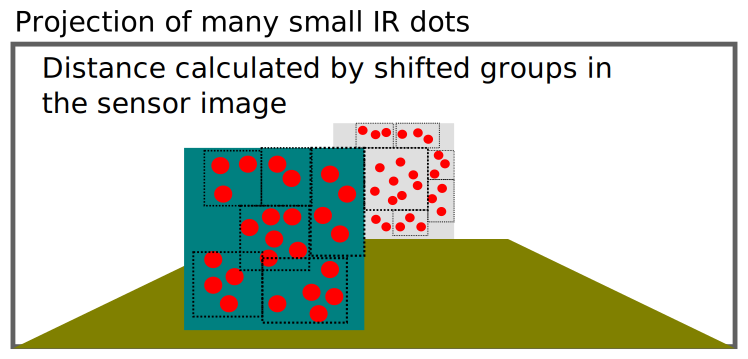
\includegraphics[scale=0.5]{kinect_principle.pdf}
	\caption{Kinect Working Principle}
	\label{figure:kinect_WP} 
\end{figure}
\clearpage

\section{Filtering}










